\documentclass{standalone}
\standaloneconfig{border=10mm}

\usepackage[
  block-border-radius=3mm,
  container-fill=nskSecondaryAccent!60,
  container-border-color=nskBlue,
]{neural-sketch}
\nskUseModule{*}

\begin{document}

\begin{nskFigure}[]
	\nskBlock[
		id=audio,
		text-north={\large \textbf{Audio}},
		width=6cm, height=1.8cm, fill=nskSecondaryAccent,
		embed-border-size=0mm,
		embed-padding=0mm, importance=1.2,
		embed={
				\node[yshift=-.4mm]
				{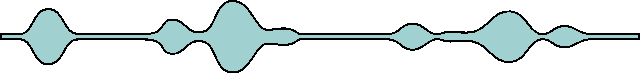
\includegraphics[width=6.1cm, height=1cm]
					{../assets/waveform.pdf};};
			},
	]
	\nskBlock[id=a, text-center=A, last-pos={below=}, width=1.2cm, height=1.2cm, fill=nskBlue]
	\nskFillBetween[from=\nskBlockIDLast{2}, to=\nskBlockIDLast{1}, edge=curved]
	\nskCoord[last-pos={below=.5cm}] % dummy coord
	\nskContainer[padding=1mm, border-radius=4mm]{
		\foreach \c in {31,...,29} {
				\nskBlock[text-center=\c, last-pos={below=1mm}, width=4cm,]
			}
		\nskBlock[text-center=1, last-pos={below=}, width=4cm,]
		\nskConnect[
			from=\nskBlockIDLast{1}, to=\nskBlockIDLast{2},
			arrow-style={dashed, very thick},
		]
		\nskBlock[text-center=Decoder, last-pos={below=}, width=4cm, fill=nskMainAccent]
		\nskConnect[
			from=\nskBlockIDLast{1}, to=\nskBlockIDLast{2},
			arrow-tip={Circle[width=2mm, length=.8mm]-Straight Barb},
			shorten-from={1mm}, shorten-to={1mm}
		]
		\nskBlock[text-center=0, last-pos={below=}, width=4cm,]
		\nskConnect[
			from=\nskBlockIDLast{1}, to=\nskBlockIDLast{2},
			arrow-tip={Circle[width=2mm, length=.8mm]-Straight Barb},
			shorten-from={1mm}, shorten-to={1mm}
		]
	}
	\nskFillBetween[from=a, to=\nskBlockIDLast{1}, edge=curved]
	\nskBlock[
		id=abt, fill=nskMainAccent,
		text-center=\Large \textbf{Autoregressive Backbone Transformer},
		width=15cm,height=2cm, last-pos={below right=1cm and -6cm},
	]
	\nskCoord[id=cx, at={abt.north}, shift-x=-3.65cm]
	\nskConnect[
		from=cx, to={\nskBlockIDLast{3}.south},
		arrow-tip={Circle[width=2mm, length=.8mm]-Straight Barb},
		shorten-to={1mm}
	]
	% abt coords ~~~~~~~~~~~~~~~~~~~~~~~~~~~~~~~~~ <<<
	\nskCoord[id=cxb, at={abt.south}, shift-x=-3.65cm]
	\nskCoord[id=cxt, at={abt.north}, shift-x=.5cm]
	\nskCoord[id=cxtb, at={abt.south}, shift-x=1cm]
	\nskCoord[id=cxtr, at={abt.north}, shift-x=2cm]
	\nskCoord[id=cxbr, at={abt.south}, shift-x=2cm]
	% abt coords ~~~~~~~~~~~~~~~~~~~~~~~~~~~~~~~~~ <<<
	% dummy coord
	\nskCoord[pos={below left=1.3cm and 1.3cm of abt}]
	\foreach \c/\f in {A/nskBlue, A/nskBlue, T/nskOrange, T/nskOrange, T/nskOrange} {
			\nskBlock[text-center=\c, last-pos={right=1mm}, fill=\f]
		}
	\nskConnect[
		from=\nskBlockIDLast{1}.north, to=cxb,
		arrow-tip={Circle[width=2mm, length=.8mm]-Straight Barb},
		shorten-from=1mm,
	]
	\nskConnect[
		from=audio.east, to=cxt,
		bend-type=single, bend-direction=down,
		arrow-style={very thick, dashed}
	]
	% right side ~~~~~~~~~~~~~~~~~~~~~~~~~~~~~~~~~ <<<
	\nskBlock[id=aa, text-center=A, pos={right=4.4cm of a}, width=1.2cm, height=1.2cm, fill=nskBlue]
	\nskCoord[last-pos={below=.5cm}] % dummy coord
	\nskContainer[padding=1mm, border-radius=4mm]{
		\foreach \c in {31,...,29} {
				\nskBlock[last-pos={below=1mm}]
			}
		\nskBlock[last-pos={below=}]
		\nskConnect[
			from=\nskBlockIDLast{1}, to=\nskBlockIDLast{2},
			arrow-style={dashed, very thick},
		]
		\nskBlock[last-pos={below=}, fill=nskMainAccent]
		\nskConnect[
			from=\nskBlockIDLast{1}, to=\nskBlockIDLast{2},
			arrow-tip={Circle[width=2mm, length=.8mm]-Straight Barb},
			shorten-from={1mm}, shorten-to={1mm}
		]
		\nskBlock[last-pos={below=}]
		\nskConnect[
			from=\nskBlockIDLast{1}, to=\nskBlockIDLast{2},
			arrow-tip={Circle[width=2mm, length=.8mm]-Straight Barb},
			shorten-from={1mm}, shorten-to={1mm}
		]
	}
	\nskConnect[
		to=\nskBlockIDLast{1}, from=cxtr,
		arrow-tip={Circle[width=2mm, length=.8mm]-Straight Barb},
		shorten-to={1mm}
	]
	\nskFillBetween[from=aa, to=\nskBlockIDLast{1}, edge=curved]
	\nskCoord[pos={right=.2cm of \nskBlockIDLast{2}}] % dummy coord
	\foreach \b/\f in {dots, A/nskBlue, A/nskBlue, A/nskBlue, T/nskOrange} {
			\begin{nskSwitch}[type=string]{\b}
				\nskCase[dots]{
					\nskBlock[
						last-pos={right=.0cm},
						border-type=none, fill=none, shadow=false,
						text-center={\tiny$\bullet\bullet\bullet$}
					]
				}
				\nskDefault{
					\nskBlock[
						last-pos={right=1mm}, text-center=\b,
						fill=\f,
					]
				}
			\end{nskSwitch}
		}
	\nskBlock[text-center=A, pos={below=.8cm of cxtb}, fill=nskBlue]
	\nskConnect[
		from=\nskBlockIDLast{1}.east, to=cxbr,
		bend-type=single, bend-direction=down,
		arrow-tip={-Straight Barb}
	]
	\nskCoord[pos={right=1.2cm of \nskBlockIDLast{1}}] % dummy coord
	\foreach \b/\f in {A/nskBlue, A/nskBlue, dots/, T/nskOrange, T/nskOrange} {
			\begin{nskSwitch}[type=string]{\b}
				\nskCase[dots]{
					\nskBlock[
						last-pos={right=.0cm},
						border-type=none, fill=none, shadow=false,
						text-center={\tiny$\bullet\bullet\bullet$}
					]
				}
				\nskDefault{
					\nskBlock[
						last-pos={right=1mm}, text-center=\b,
						fill=\f,
					]
				}
			\end{nskSwitch}
		}
	% left fade block ~~~~~~~~~~~~~~~~~~~~~~~~~~~~ <<<
	\nskBlock[
		pos={below right=-7cm and -2cm of \nskBlockIDLast{2}},
		width=2cm, height=7cm, fade=right,
	]
	\nskBlock[
		last-pos={left=13.3cm},
		width=2cm, height=7cm, fade=left,
	]
\end{nskFigure}
\end{document}
